% Digital Logic Report Template
% Created: 2020-01-10, John Miller

%==========================================================
%=========== Document Setup  ==============================

% Formatting defined by class file
\documentclass[11pt]{article}

% ---- Document formatting ----
\usepackage[margin=1in]{geometry}	% Narrower margins
\usepackage{booktabs}				% Nice formatting of tables
\usepackage{graphicx}				% Ability to include graphics				% Including multipage pdfs

%\setlength\parindent{0pt}	% Do not indent first line of paragraphs 
\usepackage[parfill]{parskip}		% Line space b/w paragraphs
%	parfill option prevents last line of pgrph from being fully justified

% Parskip package adds too much space around titles, fix with this
\RequirePackage{titlesec}
\titlespacing\section{0pt}{8pt plus 4pt minus 2pt}{3pt plus 2pt minus 2pt}
\titlespacing\subsection{0pt}{4pt plus 4pt minus 2pt}{-2pt plus 2pt minus 2pt}
\titlespacing\subsubsection{0pt}{2pt plus 4pt minus 2pt}{-6pt plus 2pt minus 2pt}

% ---- Hyperlinks ----
\usepackage[colorlinks=true,urlcolor=blue]{hyperref}	% For URL's. Automatically links internal references.

% ---- Code listings ----
\usepackage{listings} 					% Nice code layout and inclusion
\usepackage[usenames,dvipsnames]{xcolor}	% Colors (needs to be defined before using colors)

% Define custom colors for listings
\definecolor{listinggray}{gray}{0.98}		% Listings background color
\definecolor{rulegray}{gray}{0.7}			% Listings rule/frame color

% Style for Verilog
\lstdefinestyle{Verilog}{
	language=Verilog,					% Verilog
	backgroundcolor=\color{listinggray},	% light gray background
	rulecolor=\color{blue}, 			% blue frame lines
	frame=tb,							% lines above & below
	linewidth=\columnwidth, 			% set line width
	basicstyle=\small\ttfamily,	% basic font style that is used for the code	
	breaklines=true, 					% allow breaking across columns/pages
	tabsize=3,							% set tab size
	commentstyle=\color{gray},	% comments in italic 
	stringstyle=\upshape,				% strings are printed in normal font
	showspaces=false,					% don't underscore spaces
}

% How to use: \Verilog[listing_options]{file}
\newcommand{\Verilog}[2][]{%
	\lstinputlisting[style=Verilog,#1]{#2}
}




%======================================================
%=========== Body  ====================================
\begin{document}

\title{ELC 2137 Lab \#9: ALU with Input Register}
\author{Samuel Baker}

\maketitle


\section*{Summary}

The objectives of this lab were to understand and use the double-dabble algorithm to convert binary or hexadecimal values into binary coded decimal (BCD), and implement this algorithm into hardware. This was done by creating Verilog modules for an Add 3, two BCD decoders, and a top-level module used to connect to the Basys3 board. The results of all of this can be seen below. 


\section*{Q\&A}

There were no questions to answer for this experiment.

\section*{Results}

The first step of this experiment was to create an Add 3 module. As the name implies, this module adds 3 to the input, but only if it is 5 or greater, and then outputs that sum. The code for this module and its testbecnh can be found in Listings 1 and 2, and its ERT and simulation waveform can be found in Figure 1.

\begin{center}

	
	\begin{tabular}{c|ccccccccccc}
		\toprule
		Time (ns) & 0-5 & 5-10 & 10-15 & 15-20 & 20-25 & 25-30 & 30-35 & 35-40 & 40-45 & 45-50 & 50-55\\
		\midrule
		D (hex) & 0 & 0 & A & A & 3 & 3 & 0 & 0 & 0->6 & 6 & 6\\
		clk & 0 & 1 & 0 & 1 & 0 & 1 & 0 & 1 & 0 & 1 & 0\\
		en & 0 & 0 & 1 & 1 & 1->0 & 0->1 & 1->0 & 0 & 0->1 & 1 & 1\\
		rst & 0 & 0->1 & 0 & 0 & 0 & 0 & 0 & 0 & 0 & 0 & 0\\
		\midrule
		Q (hex) & X & X->0 &  & 0011 & 0100 & 1000 & 1001 & 1010 & 1011 & 1100 & 1101\\
		\bottomrule
	\end{tabular} 
	
	
	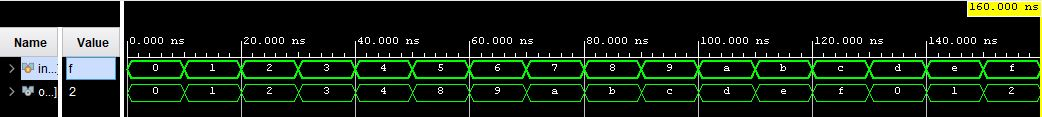
\includegraphics[width=\textwidth]{add3.jpg}
	
	Figure 1: The Add 3 ERT and Simulation Results.
\end{center}

Once this module had been constructed and had its operation confirmed by the simulation above, it was time to begin constructing BCD modules. BCD modules take a binary input and convert it into Binary Coded Decimal, which means every four bits represents one digit of a decimal number. For example, 10010011 = 93, because 1001 = 9 and 0011 = 3. BCD outputs are usually in the form of four-bit outputs of ones, tens, hundreds, and so forth. The simulation results show this most clearly, while the ERT's combine each output to get the total decimal number. These modules were constructed using cascading Add 3's. A schematic for a 6 bit-BCD can be found in Figure 2. In the Figure, C denotes an Add 3 module.

\begin{center}
	\includegraphics[width=\textwidth]{6bitBCD.jpg}

	Figure 2: The 6-bit BCD block diagram.
\end{center}

The code for the 6-bit BCD and its test bench can be found in Listings 3 and 4. The ERT and simualtion results of the 6-bit BCD can be found in Figure 3. The simulation results are in two parts, since the simulation goes on for a long time. The snippets taken are from the very beginning and the very end. This will be done as well for the rest of the simulations in the experiment.

\begin{center}
	
	\begin{tabular}{c|cccccc}
		\toprule
		Time (ns) & 0-10 & 10-20 & 20-30 & 30-40 & 40-50 & 50-60\\
		\midrule
		in0 (hex) & 0E & 0E & 0E & 0E & 0E & 0E\\
		in1 (hex) & 7A & 7A & 7A & 7A & 7A & 7A\\
		op & 0 & 1 & 2 & 3 & 4 & 0\\
		\midrule
		out (hex) & 88 & 94 & A & 7E & 74 & 88\\
		\bottomrule
	\end{tabular} 
	
	
	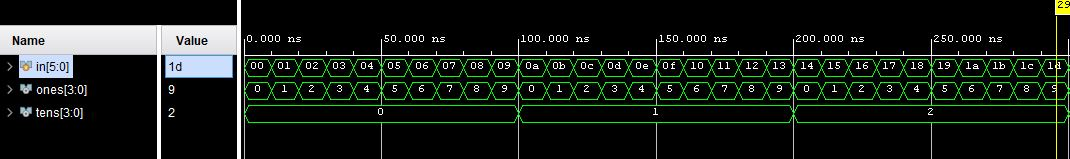
\includegraphics[width=\textwidth]{BCD_6b_beg.JPG}
	
	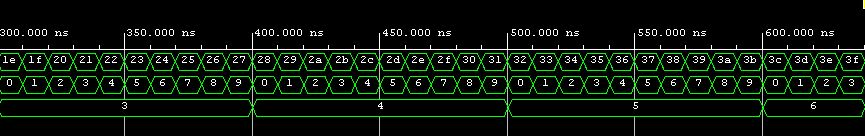
\includegraphics[width=\textwidth]{BCD_6b_end.JPG}
	
	Figure 3: The 6-bit BCD ERT and simulation results.
\end{center}


The ERT matches the simulation, therefore confirming the modules operation. The next module to be created was an 11-bit BCD. This does the exact same thing as the 6-bit BCD, but takes in 11-bits of input, therefore outputting more bits as well. A diagram of the 11-bit BCD can be found in Figure 4. 

\begin{center}

	\includegraphics[width=\textwidth]{BCD11_diagram.JPG}

	Figure 4: The 11-bit BCD module block diagram.
	
\end{center}

This diagram was then implemented into Verilog code, which can be seen in Listing 5, and tested by the testbench set in Listing 6. The ERT and simulation results for this module can be seen below in Figure 5. 

\begin{center}
	
	\begin{tabular}{c|ccccc}
		\toprule
		Time (ns) & 0 & 50 & 80 & 10,200 & 10,240\\
		\midrule
		input (hex) & 000 & 00A & 010 & 7F8 & 7FF\\
		\midrule
		output (decimal) & 0000 & 0011 & 0016 & 2040 & 2047\\
		\bottomrule
	\end{tabular} 
	
	
	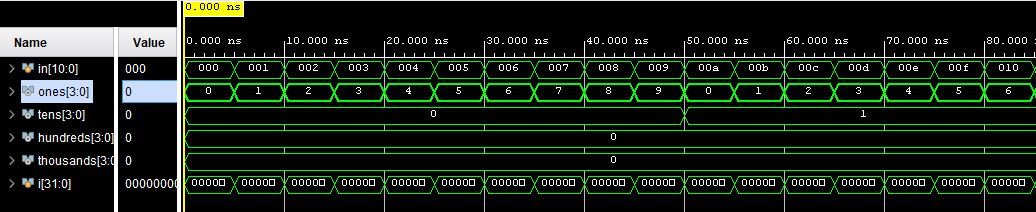
\includegraphics[width=\textwidth]{bcd11.JPG}
	
	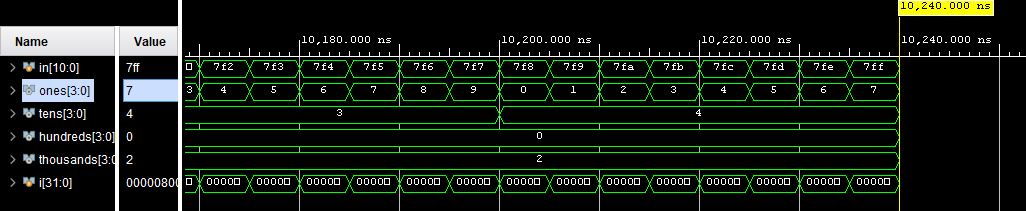
\includegraphics[width=\textwidth]{bcd11_end.JPG}
	
	Figure 5: The 11-bit BCD ERT and simulation results.
\end{center}

This ERT matches the simulation, thus verifying the 11-bit BCD's functionality. Now that both two BCD modules had been constructed, the next step in the experiment was to create a top level module that included a multiplexer and a seven segment decoder, in order to connect to the Basys3 board. This would be similar to the seven-segment decoder constructed in the last lab, but with the added functionality of a 11-bit BCD, which would restrict the board to only displaying decimal numbers. A diagram of this module is included in Figure 6.


\begin{center}
	\includegraphics[width=1\textwidth]{sseg_diagram.JPG}
	
	Figure 6: The seven segment display module block diagram.
	
	
\end{center}

The code for this module can be found in Listing 7. Once this module had been constructed, the Basys3 board was connected to the computer. Once connected, a bit stream was generated in Vivado and the board was programmed to use the seven segment display module previously mentioned. The board was then turned on and the switches were set in order to display "98" on the board. The results of which can be seen below in Figures 7 and 8.

\begin{center}
	\includegraphics[width=1\textwidth]{IMG-4527.jpg}
	
	Figure 7: Working seven-segment display displaying 8 for the "ones" spot.
	
	\includegraphics[width=1\textwidth]{IMG-4528.jpg}
	
	Figure 8: Working seven-segment display displaying 9 for the "tens" spot.
	
	
\end{center}

As can be seen through all of the above modules and simulations, the dibble-dabble algorithm was succesfully implemented in code, and then in hardware, to achieve a working BCD seven segment display. This brought forth a greater understanding of the algorithm and how to generally implement algorithms into hardware, therfore fulfilling the objectives of the experiment.


\clearpage

\section*{Code}

Below are the listings containing all of the code written in this experiment.

\Verilog[caption=Code for the Add 3 module]{add3.sv}

\Verilog[caption=Code for the Add 3 Testbench]{add3_test.sv}

\clearpage

\Verilog[caption=Code for the 6-bit BCD module]{BCD_6b.sv}

\clearpage

\Verilog[caption=Code for the 6-bit BCD Testbench]{BCd_6b_test.sv}

\clearpage

\Verilog[caption=Code for the 11-bit BCD module]{bcd11.sv}

\clearpage

\Verilog[caption=Code for the 11-bit BCD Testbench]{bcd11_test.sv}

\clearpage

\Verilog[caption=Code for the seven-segment top level module]{sseg1_BCD.sv}


\end{document}
